% -----------------------------------------------------------------------------
% E3 results update: final 160M run and 410M scale check
% -----------------------------------------------------------------------------
% Suggested location: Chapter 4, after E1/E2 and before optional E4/E5/E6.

\section{E3: stage-dependent durability of injected factual signal}
\label{sec:results-e3-final}

E3 tests the central causal prediction of the thesis.  E1 located an early weight-space reorganisation window independently from spectral indicators, and E2 showed that this interval overlaps with rapid functional improvement.  E3 asks whether that same interval is also a period of greater durable plasticity: after injecting the same novel factual signal into checkpoints from different stages, does the signal survive subsequent training pressure better when it is injected near the reorganisation window?

\subsection{Primary 160M run}
\label{sec:results-e3-160m}

The primary run used \texttt{EleutherAI/pythia-160m-deduped} at eight checkpoints: steps 0, 128, 512, 1000, 2000, 3000, 8000, and 143000.  For each checkpoint I ran five independently generated factual-signal seeds, giving 40 cells.  Each cell injected 300 synthetic factual associations, measured immediate uptake on held-out paraphrase probes, continued training on the same fixed Pile-validation corpus, and separately measured overwrite resistance under nested conflicting-fact poison budgets.

The signal entered the model at every stage.  All 40 cells had positive uptake by log-probability margin, with mean uptake margin delta $1.785$.  Uptake was not perfectly matched across stages: the final checkpoint learned the synthetic facts with much larger immediate margin than the early checkpoints.  Therefore, raw post-injection scores and raw post-poison scores are not the primary durability outcomes.  The main analysis uses uptake-normalised retention and uptake-normalised degradation resistance.

\begin{figure}[t]
    \centering
    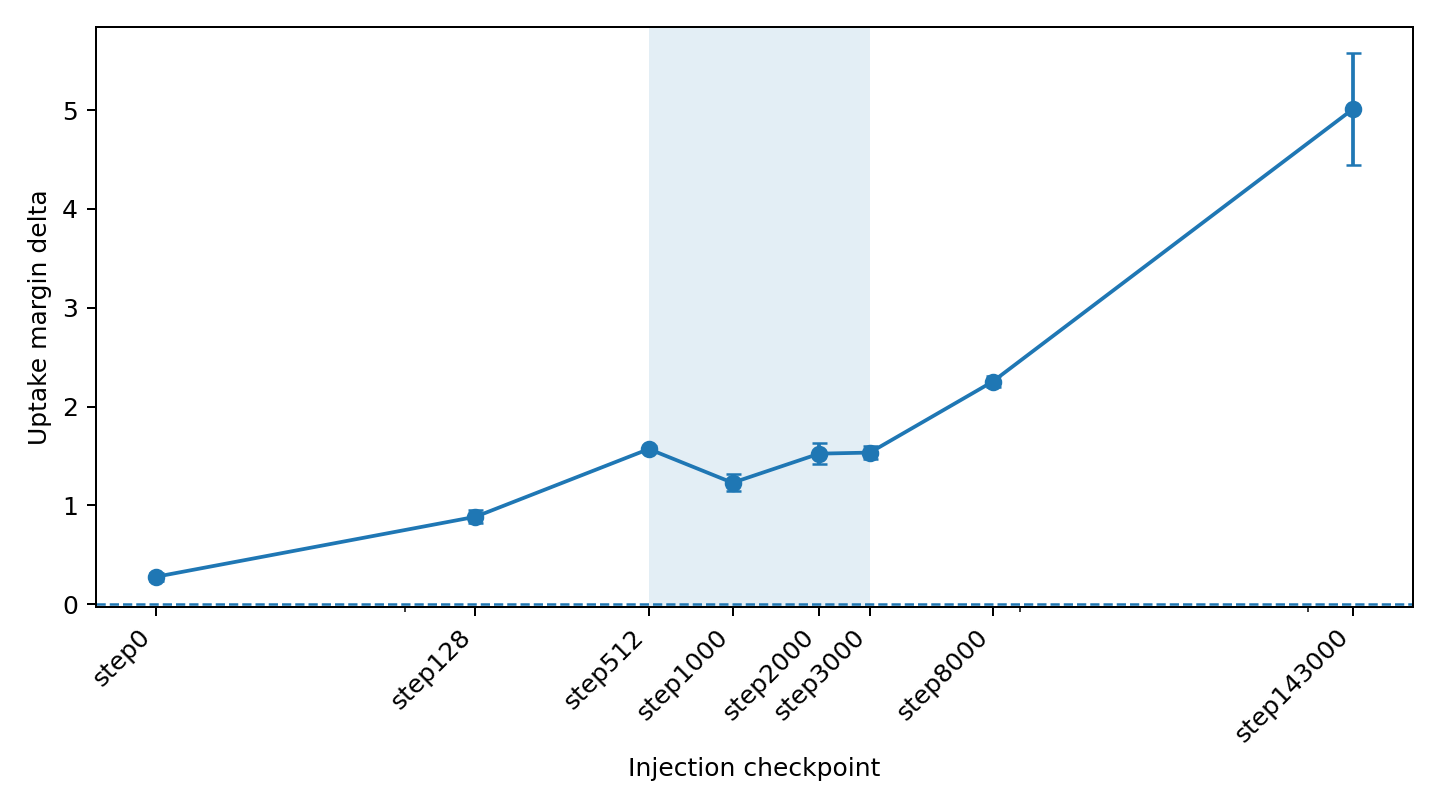
\includegraphics[width=0.78\linewidth]{figures/e3/e3_uptake_margin_by_stage.png}
    \caption{E3 uptake in the primary Pythia-160M run.  The synthetic factual signal is learned at all stages, but uptake is larger at late checkpoints.  This motivates the use of uptake-normalised durability metrics.}
    \label{fig:e3-160m-uptake}
\end{figure}

The clean-continuation branch gives the clearest evidence for stage-dependent durability.  Mean uptake-normalised margin retention by stage was:
\[
\begin{array}{c|rrrrrrrr}
\text{stage} & 0 & 128 & 512 & 1000 & 2000 & 3000 & 8000 & 143000 \\
\hline
R_M & -1.37 & 0.34 & 0.61 & 0.76 & 0.67 & 0.63 & 0.46 & 0.25 .
\end{array}
\]
The step-0 value is treated as a diagnostic baseline rather than as part of the stage-window comparison, because the untrained checkpoint behaves qualitatively differently.  Among trained checkpoints, retention peaks around steps 1000--2000, close to the independently located E1 boundary.

A window-versus-late comparison makes the pattern clearer.  The E1/E2 window checkpoints, defined as steps 512, 1000, 2000, and 3000, retained on average approximately $0.67$ of the injected margin after fixed Pile continuation.  The late checkpoints, steps 8000 and 143000, retained approximately $0.35$.  Thus, the same signal is not merely easier to inject near the window; after normalising for how much signal entered, a larger fraction of it survives subsequent generic training pressure.

\begin{figure}[t]
    \centering
    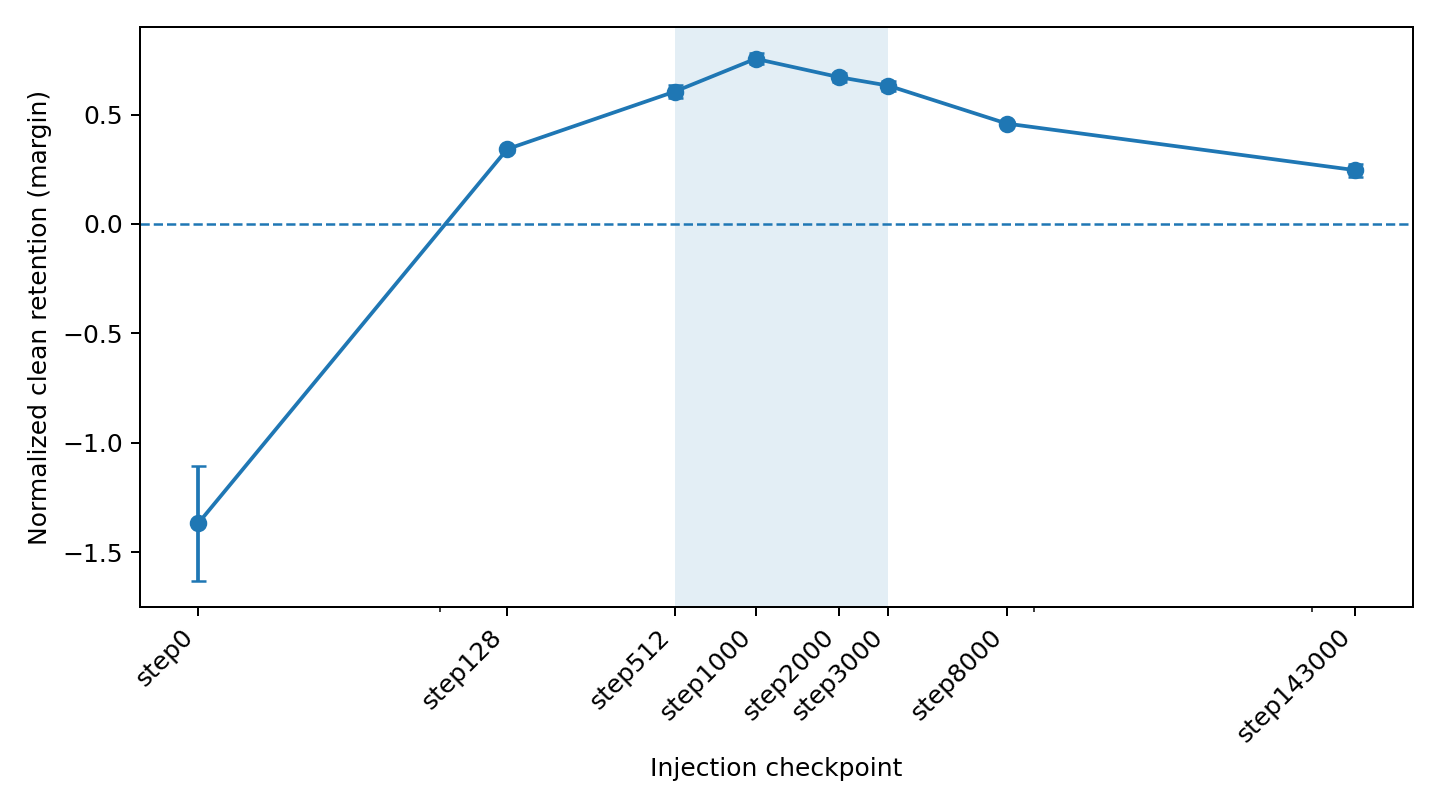
\includegraphics[width=0.78\linewidth]{figures/e3/e3_normalized_retention_margin_by_stage.png}
    \caption{Uptake-normalised clean retention in the primary Pythia-160M E3 run.  Retention is highest near the E1/E2 reorganisation window and lower at later consolidated checkpoints.}
    \label{fig:e3-160m-normalized-retention}
\end{figure}

The conflicting-fact degradation branch points in the same broad direction, although it is less sharply boundary-like than clean retention.  Mean uptake-normalised degradation AUC is highest in the 512--3000 range and lowest at the final checkpoint.  This suggests that overwrite resistance also declines after consolidation, but the effect is more gradual than the clean-retention result.

\begin{figure}[t]
    \centering
    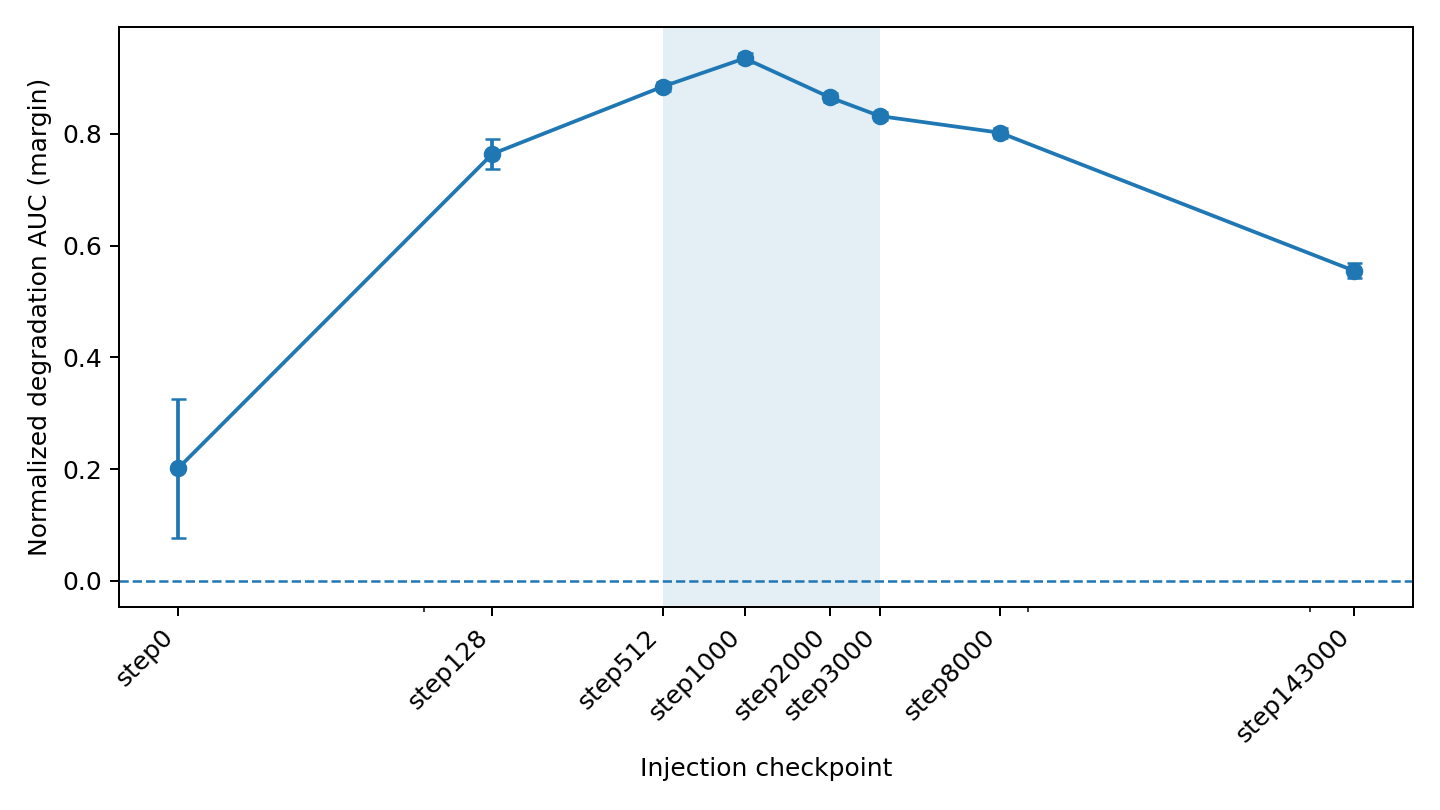
\includegraphics[width=0.78\linewidth]{figures/e3/e3_normalized_degradation_auc_margin_by_stage.png}
    \caption{Uptake-normalised degradation resistance in the primary Pythia-160M E3 run.  Higher values indicate that more of the injected margin survives conflicting-fact overwrite.  The curve broadly agrees with the clean-retention result, but the decline is more gradual.}
    \label{fig:e3-160m-normalized-degradation}
\end{figure}

The 160M result therefore supports the central E3 prediction in its short-horizon form.  The candidate window was identified independently from weight-space spectra in E1; E3 shows that a behavioural durability measure is highest near that window and lower after consolidation.  The result should be described as evidence for a short-horizon sensitive period, not as proof of a strong critical period: the experiment uses checkpoint fine-tuning and a fixed continuation budget, not continuation to the end of pre-training.

\subsection{410M scale-check replication}
\label{sec:results-e3-410m}

To test whether the pattern was specific to Pythia-160M, I ran the same factual-intervention protocol on \texttt{EleutherAI/pythia-410m-deduped}.  This run used the same eight stages but three seeds per stage, giving 24 cells.  Uptake was positive in 23 of 24 cells.  The earliest stages, especially step 0 and partly step 128, are again best treated as diagnostic baselines because uptake is weak there.

The 410M run qualitatively replicates the 160M result.  Mean uptake-normalised clean retention was:
\[
\begin{array}{c|rrrrrrrr}
\text{stage} & 0 & 128 & 512 & 1000 & 2000 & 3000 & 8000 & 143000 \\
\hline
R_M & -0.94 & -0.08 & 0.54 & 0.74 & 0.75 & 0.71 & 0.51 & 0.41 .
\end{array}
\]
The same peak appears around steps 1000--2000, and the same decline appears at later checkpoints.  Averaging over the 512--3000 window gives mean normalised margin retention of approximately $0.67$, compared with approximately $0.45$ for the late 8000/final checkpoints.  The paired seed-level window-minus-late difference is positive for all three seeds.

\begin{figure}[t]
    \centering
    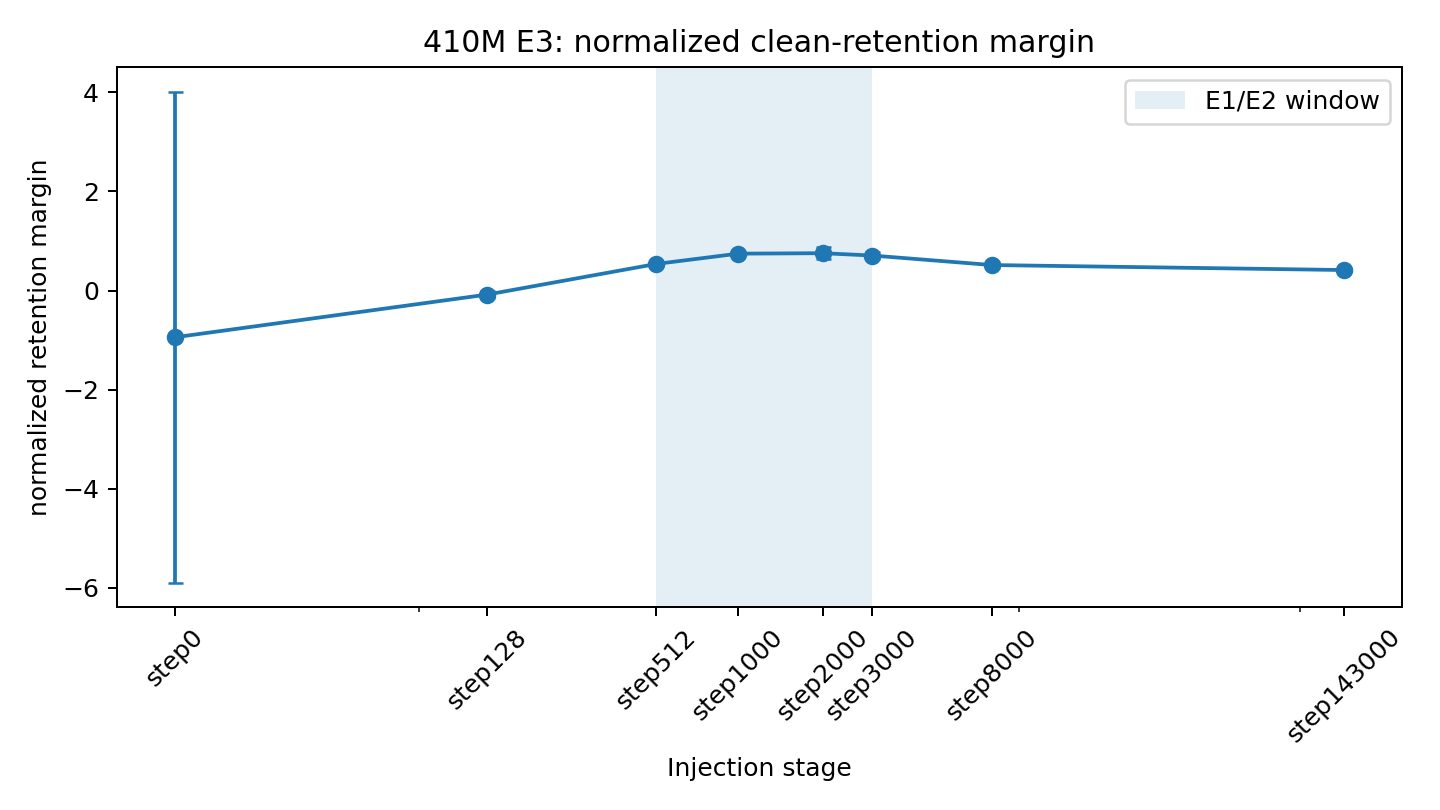
\includegraphics[width=0.78\linewidth]{figures/e3/e3_410m_normalized_retention_margin_by_stage.png}
    \caption{Uptake-normalised clean retention in the Pythia-410M reduced scale check.  The 410M run reproduces the 160M pattern: injected signal is retained best near the E1/E2 reorganisation window and less at late checkpoints.}
    \label{fig:e3-410m-normalized-retention}
\end{figure}

The 410M degradation branch also agrees in direction.  Mean normalised degradation AUC is approximately $0.82$ in the 512--3000 window and approximately $0.61$ at late checkpoints.  As in the 160M run, degradation resistance is a supporting measure rather than the cleanest headline result.

\begin{figure}[t]
    \centering
    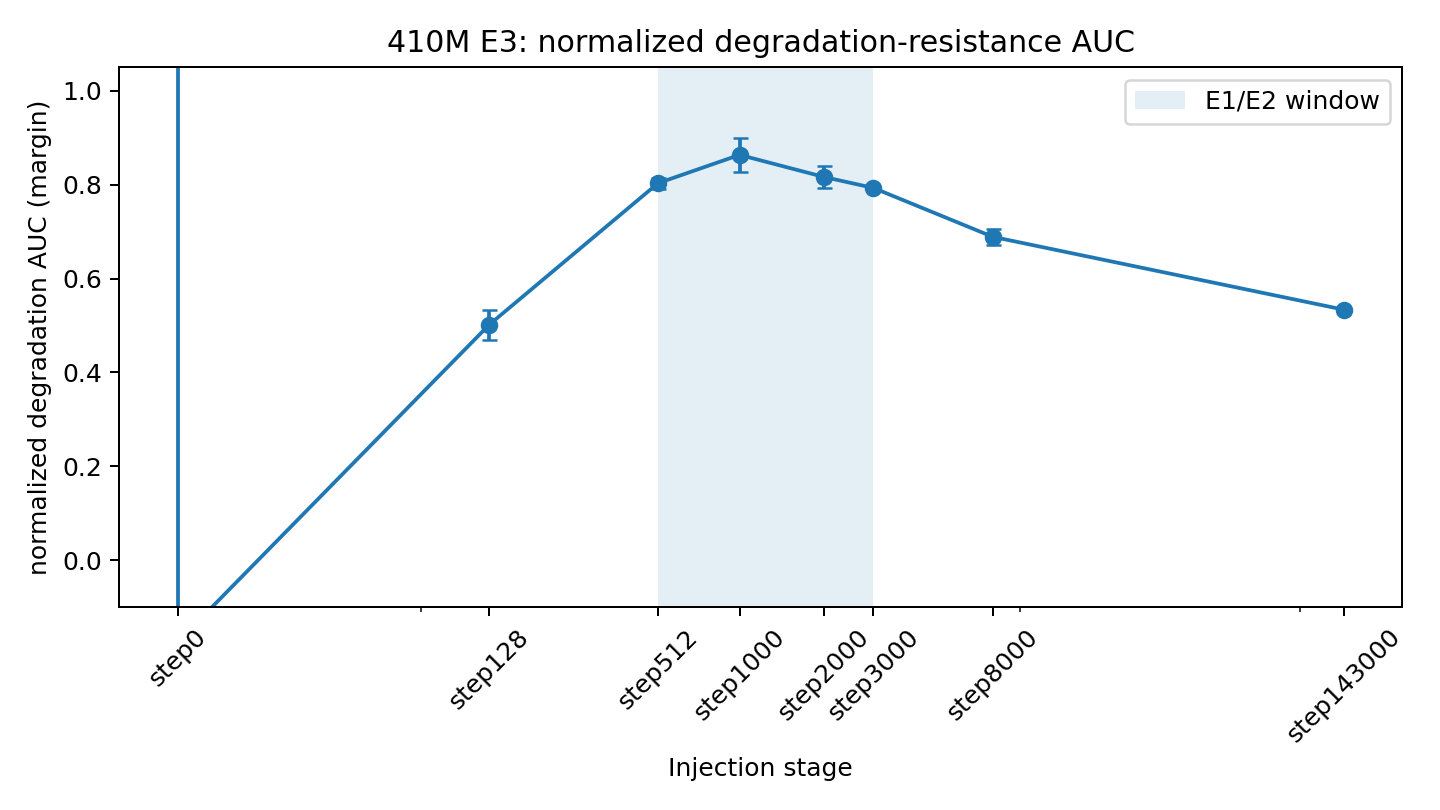
\includegraphics[width=0.78\linewidth]{figures/e3/e3_410m_normalized_degradation_auc_margin_by_stage.png}
    \caption{Uptake-normalised degradation resistance in the Pythia-410M scale check.  The overwrite-resistance measure is highest around the reorganisation window and lower at late checkpoints.}
    \label{fig:e3-410m-normalized-degradation}
\end{figure}

\subsection{Interpretation of E3}
\label{sec:results-e3-interpretation}

Taken together, the 160M full run and 410M reduced scale check provide evidence that the early reorganisation window identified in E1 is functionally consequential for short-horizon durability.  The strongest result is not raw uptake: late checkpoints can learn the synthetic facts strongly under the fixed fine-tuning budget.  The stronger result is uptake-normalised durability.  Conditional on the signal entering the model, more of the injected margin survives fixed Pile continuation when injected near steps 512--3000, especially around steps 1000--2000, than when injected after consolidation.

This result rules out several trivial interpretations by design.  The injection learning rate is fixed across stages, so the pattern is not simply inherited from the natural pre-training learning-rate schedule.  The clean-continuation corpus and continuation budget are fixed across stages, so the pattern is not due to early checkpoints receiving more or different post-injection training.  The signal is synthetic and novel, so the pattern is not due to prior factual knowledge.  Finally, uptake is measured directly and durability is normalised by uptake.

The appropriate conclusion is therefore cautious but positive: E3 supports a short-horizon sensitive-period interpretation in small Pythia models.  It does not prove lifetime persistence, and it does not by itself establish a biological-style critical period.  But it does show that the independently identified E1/E2 reorganisation window predicts a behavioural durability difference under controlled checkpoint intervention.
